\section{Approximate operations terms}

We introduce some new terms: aproximate sum, difference and inverse. The names come from dilation structures, Definition 11 \cite{buligadil1},  where they play an important role. 



\begin{definition}
The asum (approximate sum), adif (approximate difference) and ainv (approximate inverse) are the terms: 
\begin{enumerate}
\item[-] asum or approximate sum, for $a \in \Upsilon$: $\displaystyle \Sigma_{a}^{e}(x,y) \, = \, \bar{a}^{e} a^{a^{e} x} y$

\centerline{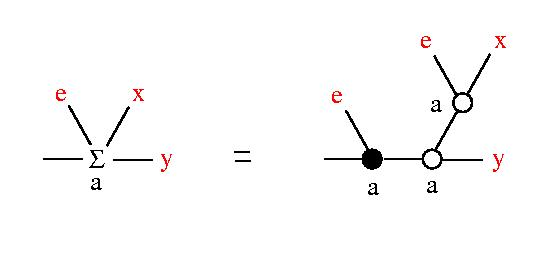
\includegraphics[width=80mm]{jpg/asum.jpg}}  
\item[-] adif or approximate difference, for $a \in \Upsilon$: $\displaystyle \Delta_{a}^{e}(x,y) \, = \, \bar{a}^{a^{e} x} a^{e} y$

\centerline{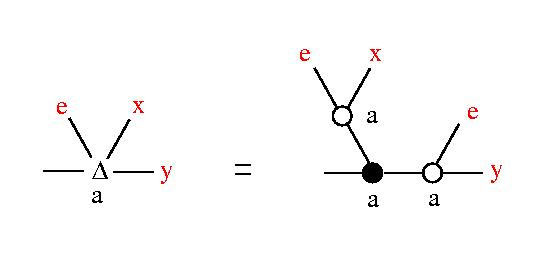
\includegraphics[width=80mm]{jpg/adif.jpg}}  
\item[-] ainv or approximate inverse, for $a \in \Upsilon$: $\displaystyle inv_{a}^{e} x \, = \, \bar{a}^{a^{e} x} e$

\centerline{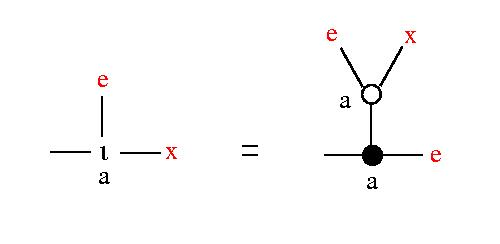
\includegraphics[width=80mm]{jpg/ainv.jpg}}  
\end{enumerate}
\label{aterms}
\end{definition}

We should think about the adif $\displaystyle \Delta_{a}^{e}(x,y)$ as the approximate difference of the vectors $-(e,x)+(e,y)$, based at $e$, and similarly about the asum or ainv. This is not needed in this general setting, but it is a good guide for the intuition of the reader. 

This analogy can be used to clarify the difference between the substraction $a - b$, with $a$ a node variable and $b$ a binary term, and the adif. We saw that, in the frame of real vector spaces and their associated irqs,  moreover with $e=0$ (the null vector of the vector space) for simplicity, 
$$\displaystyle (a-b)^{e} x \mbox{  is like }   (a-b)x$$
 In the same frame  
$$\displaystyle \Delta_{a}^{e}(x,y) \mbox{ is like } -(1-a)x + y$$
which is approximately $\displaystyle -x+y = y-x$. 

These asum, adif, ainv give to the terms a structure of an approximate conical group \cite{buligainf}, which can be informally described as an (approximate) non-commutative vector space. 
More precisely, by using the rewrites we have at our disposal, we can prove that the terms asum, adif, seen as binary operations, and ainv, seen as an unary operation, satisfy relations akin to associativity of the (vector) addition, the adif is an inverse to asum just like difference is the inverse of the sum, etc. These has been proved as identities several times, the ones we may need in this article are collected, for example, in Proposition 4.3 (a)--(g) \cite{buligabraided}, first time proved in Section 4.2  Definition 11 \cite{buligadil1}. 

As an example, the approximate associativity of asum is the statement: for any $a \in \Upsilon$ 
$$ \Sigma_{a}^{e}\left( \Sigma_{a}^{e}\left(x,y\right), z\right) \, \longleftrightarrow \, \Sigma_{a}^{e}\left( x, \Sigma_{a}^{a^{e} x} \left( y,z\right)\right) $$
whose proof is given in the Figure \ref{sumassoc}. 
\begin{figure}[h]\centerline{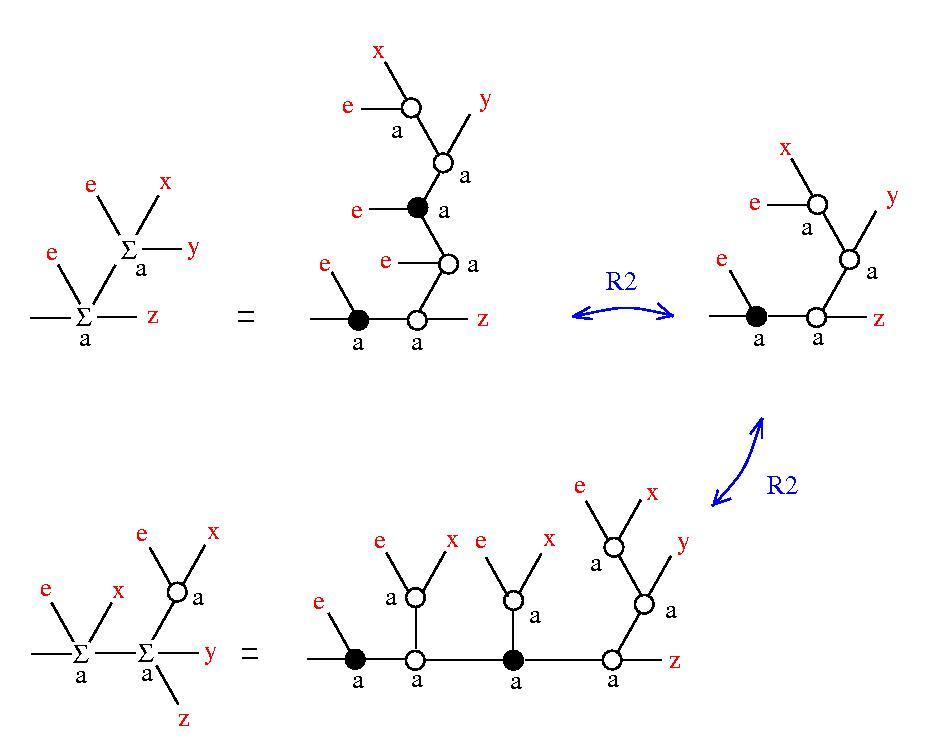
\includegraphics[width=120mm]{jpg/sumassoc.jpg}}  \caption{ The associativity of asum } \label{sumassoc} \end{figure}
